\documentclass[11pt]{article}            % Report class in 11 points
\parindent0pt  \parskip10pt             % make block paragraphs
\usepackage{graphicx}
\usepackage{listings}
\newcommand\tab[1][1cm]{\hspace*{#1}}
\usepackage[document]{ragged2e}
\usepackage{float}
\graphicspath{ {images/} }
\usepackage{graphicx} %  graphics header file
\begin{document}
\begin{titlepage}
    \centering
  \vfill
    
\includegraphics[width=8cm]{uni_logo.png} \\ 
	\vskip2cm
    {\bfseries\Large
	Data Structure and Algorithm \\ (CS09203)\\
	
	\vskip2cm
	Lab Report 
	 
	\vskip2cm
	}    

\begin{center}
\begin{tabular}{ l l  } 

Name: & Muhammad Umer \\ 
Registration \#: & CSU-F16-104 \\ 
Lab Report \#: & 01 \\ 
 Dated:& 26-03-2018\\ 
Submitted To:& Mr. Usman Ahmed\\ 

 %\hline
\end{tabular}
\end{center}
    \vfill
    The University of Lahore, Islamabad Campus\\
Department of Computer Science \& Information Technology
\end{titlepage}


    
    {\bfseries\Large
\centering
	Experiment \# 1 \\

Introduction to Arrays and its operation\\
	
	}    
 \vskip1cm
 \textbf {Objective}\\ The objectives of this lab session are to understand the basic and various operations on arrays in C++.
 
 \textbf {Software Tool} \\
1.  Window 7 (32-bit)\\
2. Sublime Text Editor\\
3. Dev C++\\

\textbf{Theory }  \\            
We have already studied array in our computer programming course. We would be using the knowledge we learned there to implement different operation on arrays. \\

\textbf{Traversing Linear Arrays:-}\\
Let A be the collection of data elements stored in the memory of the computer. Suppose we want to print the contents of each element of A or suppose we want to count the number of elements of A with a given property. This can be accomplished by traversing A that is by accessing and Processing each element of A exactly once.\\~\\
 The following algorithm traverses a linear array. The simplicity of the algorithm comes from the fact that LA is a linear structure. Other linear structures such as linked list can also be easily
traversed. On the other hand the traversal of non-linear structures such as trees and graphs is considerably more complicated.\\

\textbf{Algorithm:-}\\
(Traversing a Linear Array) Here LA is a linear Array with lower Bound LB and upper Bound
UB. This algorithm traverses LA.\\~\\
Applying an operation PROCESS to each element of LA.\\

\begin{lstlisting}[language=C++]
[Initialize Counter] Set X=LB.
	1. Repeat Step 3 and 4 while K<=UB.
	[Visit element] Apply PROCESS to LA[X].
	[Increase Counter] Set X=X+1.
	[End of Step 2 Loop]
	5. Exit.
\end{lstlisting}

\textbf{Inserting and Deleting:-}\\
Let A be a collection of data elements in the memory of computer. “Inserting” refers to the
operation of adding another element to the collection A and “deleting” refers to the operation of
removing one of the elements from A. Here we discuss the inserting and deleting when A is a
linear array.\\~\\
Inserting an element at the “end” of the linear array can be easily done provided the memory space
allocated for the array is large enough to accommodate the additional element. On the other hand
suppose we need to insert an element in the middle of the array. Then on average half of the
elements must be moved downward to the new location to accommodate the new element and keep
the order of other elements.\\~\\
Similarly deleting the element at the “end” of an array presents no difficulties but deleting the
element somewhere in the middle of the array would require that each subsequent element be
moved one location upward in order to fill up the array.\\

\textbf{Algorithm of Insertion operation:-}\\
(Inserting into Linear Array) INSERT (LA, N, K, ITEM)\\~\\
Here LA is a linear array with N elements and K is a positive integer such that K≤N. This algorithm
inserts an element ITEM into the Kth position in LA.\\


\begin{lstlisting}[language=C++]
1.[Initialize Counter] Set J=N.
2.Repeat Step 3 and 4 while J≥K.
3.		[Move Jth element downward] Set LA [J+1] =LA[J].
4.		[Decrease Counter] Set J=J-1.
	End of Step 2 Loop.
5.[Insert element] Set LA[K]=ITEM.
6.[Reset N] Set N=N+1.
7.Exit.
\end{lstlisting}

\textbf{Lab Task:-}\\
Write a C++ program to implement all the above described algorithms and display the following
menu and ask the user for the desired operation.\\
\begin{figure}[H]
\centering
  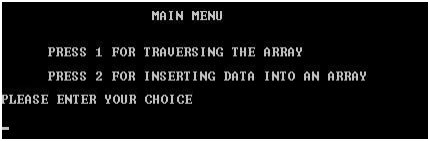
\includegraphics[width=12cm,height=6cm,keepaspectratio]{1.png}
\caption{The ouput of the program}
\label{Figure:1}    
\end{figure}
The program should have the option for reusing it after you have completed the desired task.\\


\textbf{Solution:-}\\
\begin{lstlisting}[language=C++]
#include<iostream>
#include<conio.h>
using namespace std;
void travers_array(int array[], int n){
	cout<<"\n\n";
	for(int x=0; x<n; x++)
	{
		cout<<array[x]<<" ";
	}
	cout<<"\n\nPRESS ANY KEY TO CONTINUE...";
	getch();
}

void insert(int array[],int& n, int k, int item){
	for(int j=n; j>=k; j--){
		array[j+1] = array[j];
	}
	array[k] = item;
	n = n+1;
	cout<<"\nVALUE ADDED SUCCESSFULLY";
	cout<<"\n\nPRESS ANY KEY TO CONTINUE...";
	getch();
}

void delete_value(int array[], int& n, int k){
	for(int j=k; j<=sizeof(array); j++){
		array[j] = array[j+1];
	}
	n = n-1;
	cout<<"\nVALUE DELETED SUCCESSFULLY";
	cout<<"\n\nPRESS ANY KEY TO CONTINUE...";
	getch();
}
int main()
{
	int choice,n = 5,arr[n],location,value;
	cout<<"\t\t\tENTER 5 ELEMENTS\n\n";
	for(int i=0; i<5; i++)
	{
		cout<<"Enter "<<i+1<<" Value: ";
		cin>>arr[i];
	}
	up:
	system("cls");
	cout<<"\t\t\tMAIN MENU\n\n";
	cout<<"\tPRESS 1 FOR TRAVERSING THE ARRAY\n\n";
	cout<<"\tPRESS 2 FOR INSERTING DATA INTO ARRAY\n\n";
	cout<<"\tPRESS 3 FOR DELETING DATA FROM ARRAY\n\n";
	cout<<"\tPRESS 4 TO EXIT\n\n";
	cout<<"PLEASE ENTER YOUR CHOICE\n\n";
	cin>>choice;
	if(choice == 1){
		travers_array(arr, n);
		goto up;
	}
	else if(choice == 2){
		cout<<"\n\nENTER LOCATION TO INSERT: ";
		cin>>location;
		cout<<"\nENTER VALUE TO INSERT: ";
		cin>>value;
		insert(arr, n, location-1, value);
		goto up;
	}
	else if(choice == 3){
		cout<<"\n\nENTER LOCATION TO DELETE: ";
		cin>>location;
		delete_value(arr, n, location-1);
		goto up;
	}
	else if(choice == 4){
		exit(0);
	}
	else{
		cout<<"\n\nWRONG CHOICE!";
		cout<<"\n\nPRESS ANY KEY TO CHOOSE AGAIN...";
		getch();
		goto up;
	}
	return 0;
}
\end{lstlisting}

\textbf{Output:-}
\begin{figure}[H]
\centering
  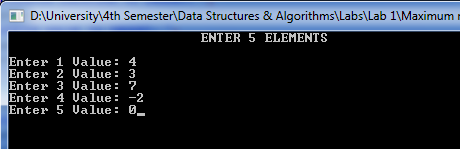
\includegraphics[width=12cm,height=6cm,keepaspectratio]{2.png}
\caption{Getting input in the start}
\label{Figure:2}    
\end{figure}

\begin{figure}[H]
\centering
  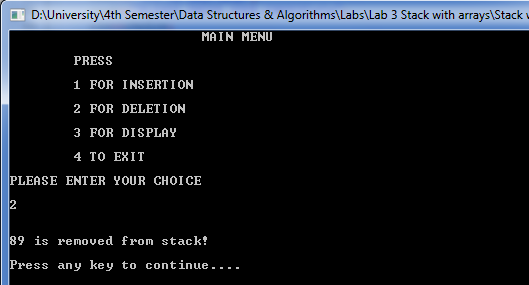
\includegraphics[width=12cm,height=6cm,keepaspectratio]{3.png}
\caption{Main Menu and Traversing the array}
\label{Figure:3}    
\end{figure}

\begin{figure}[H]
\centering
  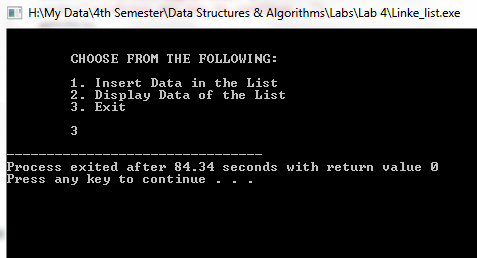
\includegraphics[width=12cm,height=6cm,keepaspectratio]{4.png}
\caption{Inserting item in the array}
\label{Figure:4}    
\end{figure}

\begin{figure}[H]
\centering
  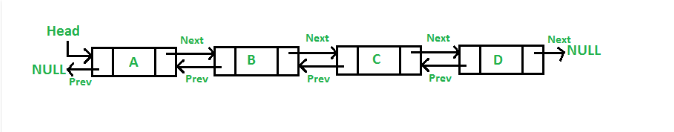
\includegraphics[width=12cm,height=6cm,keepaspectratio]{5.png}
\caption{Traversing after inserting in the array}
\label{Figure:5}    
\end{figure}

\begin{figure}[H]
\centering
  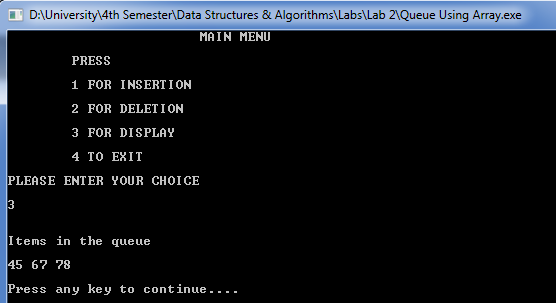
\includegraphics[width=12cm,height=6cm,keepaspectratio]{6.png}
\caption{Deleting item from the array}
\label{Figure:6}    
\end{figure}

\begin{figure}[H]
\centering
  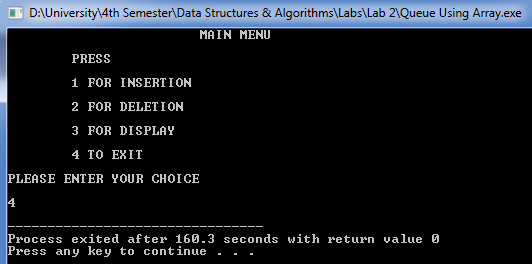
\includegraphics[width=12cm,height=6cm,keepaspectratio]{7.png}
\caption{Traversing after deleting from array}
\label{Figure:7}    
\end{figure}

\begin{figure}[H]
\centering
  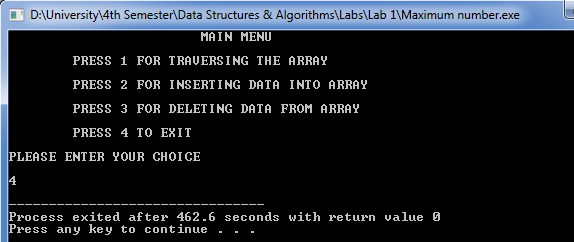
\includegraphics[width=12cm,height=6cm,keepaspectratio]{8.png}
\caption{Exit}
\label{Figure:8}    
\end{figure}

\textbf{Source Code:-}
https://github.com/umerayan/Semester-4-Labs.git\\~\\

\textbf{Conclusion:-}
Operations on arrays is a good practice to start learning Data Structures. We have already studied array in our computer programming course. In this lab we have performed different operations on arrays i.e. insertion, deletion and traversing. The above program can perform all these three operations on arrays. The program is coded in C++ and open source for everyone to use at my github account (The Link provided above) \\~\\~\\

\tab[6cm] \noindent\rule{6cm}{0.4pt}\\
\tab[6cm] (Concerned Teacher/Lab Engineer)
 
\end{document}                          % The required last line
